\section{Results}
\subsection{Coverage, abstention, and alternative retention}
Table~\ref{tab:coverage} reports every primary cell. ChronoTrace verifies all 72 FP32 observations, whereas ranked replay reaches nine matching histories at the same gradient-work budgets. At FP16, all 48 observations with durations 5 and 10 are verified, but no observation at duration 20 is verified. Ranked replay instead succeeds in eight of those 24 strong-FP16 cases. Thus the new method does not dominate ranked retrieval across the entire grid.

\begin{table}[t]
\centering
\caption{Primary results. Each row has 24 observations (12 seed clusters and two task families). ``Verified'' includes conditional uniqueness and numerical replay consistency; ``retrieved'' is a first match. Both exports observe the same 72 endpoints.}\label{tab:coverage}
\begin{tabular}{llrrr}
\toprule
Export & Duration & ChronoTrace verified & Ranked retrieved & Secant verified\\
\midrule
FP32 & 5 & 24/24 & 3/24 & 0/24\\
FP32 & 10 & 24/24 & 3/24 & 0/24\\
FP32 & 20 & 24/24 & 3/24 & 0/24\\
FP16 & 5 & 24/24 & 3/24 & 0/24\\
FP16 & 10 & 24/24 & 3/24 & 0/24\\
FP16 & 20 & 0/24 & 8/24 & 0/24\\
\midrule
Total & & 120/144 & 23/144 & 0/144\\
\bottomrule
\end{tabular}
\end{table}
Across all primary observations, 3,360 of 4,032 possible unordered-pair relations are inferred, with no observed wrong pair or full-order output. All reference-compatible orders are retained. The exhaustive compatible set is a singleton for every problem/export pair, including every strong-FP16 failure. The latter failures therefore demonstrate limited pruning under the implemented uncertainty bounds and replay cap, not established information-theoretic non-identifiability.

At duration 20 with FP16 export, all 40,320 middle candidates survive in these runs; the replay cap permits 3,125 suffixes and leaves 37,195 untested candidates. No common pairwise relation is then reported. Their unique exhaustive solutions remain present. Across the primary study, mean training-loss reduction ranges from 9.03\% to 39.53\%, and held-out classification accuracy ranges from 73.33\% to 87.78\%. These measures exclude the interpretation that the primary successes concern only infinitesimal parameter updates.

For FP32, the paired coverage difference relative to ranked first-match retrieval is 87.5 percentage points. A descriptive bootstrap resamples the 12 seed clusters with replacement, preserving all conditions within each selected cluster; 20,000 replicates with seed 55167 give a percentile interval of 76.4--97.2 points. This interval describes variation among the sampled seed clusters on a fixed dataset. It is not a guarantee over independent datasets or realistic pipelines. Zero observed mistakes likewise does not establish a population error rate of zero.

\subsection{Gradient work and runtime}
Table~\ref{tab:work} separates work from success. FP32 total work is a median of approximately $4.01\times10^5$ gradients, versus 3,507,200 for complete prefix-cached replay. The median exhaustive/new ratio is 8.74, ranging from 8.21 to 9.14. No endpoint-reference acquisition is hidden in the new decoder's budget. FP16 work increases when uncertainty leaves more candidate replays; this additional spending still fails to verify the strongest cell.

\begin{table}[t]
\centering
\caption{Median total gradient evaluations and maximum inverse radius within each observation, aggregated by cell. Prefix, inverse, residual-check, and verification work are included. The exhaustive reference uses 3,507,200 gradients in every cell.}\label{tab:work}
\begin{tabular}{llrr}
\toprule
Export & Duration & Median gradients & Median inverse radius\\
\midrule
FP32 & 5 & 384,015.5 & $1.36\times10^{-6}$\\
FP32 & 10 & 401,366.0 & $3.38\times10^{-5}$\\
FP32 & 20 & 415,942.0 & $1.67\times10^{-2}$\\
FP16 & 5 & 384,706.5 & $1.11\times10^{-2}$\\
FP16 & 10 & 447,889.0 & $2.76\times10^{-1}$\\
FP16 & 20 & 714,252.5 & $1.36\times10^{2}$\\
\bottomrule
\end{tabular}
\end{table}

The eight serial timing pairs yield a median ChronoTrace time of 1.824 seconds and a median exhaustive time of 13.214 seconds. The median of the paired ratios is 7.33, with a range of 6.70--15.46. The largest ratio includes a 25.93-second exhaustive run; retaining this outlier avoids selective reporting, and the paired median reduces its influence. All repeated outputs agree with the exhaustive reference. These are same-environment repeat checks on spent inputs, not new independent confirmation. Timings do not establish an asymptotic speedup, and machine-specific performance should be remeasured with recorded hardware.

\begin{figure}[t]
\centering
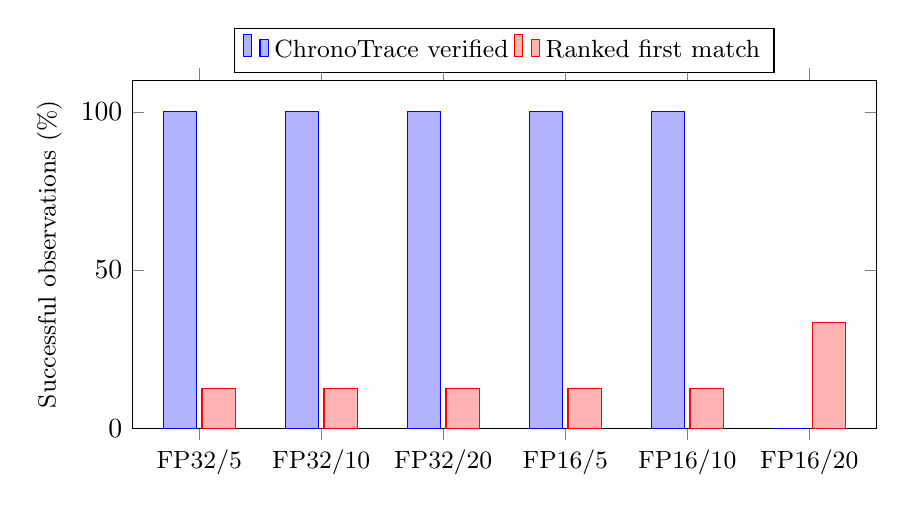
\begin{tikzpicture}
\begin{axis}[width=.91\linewidth,height=6.0cm,ybar,bar width=12pt,
 ymin=0,ymax=110,ylabel={Successful observations (\%)},
 symbolic x coords={32/5,32/10,32/20,16/5,16/10,16/20},xtick=data,
 xticklabels={FP32/5,FP32/10,FP32/20,FP16/5,FP16/10,FP16/20},
 x tick label style={font=\small},ylabel style={font=\small},
 legend style={at={(.5,1.02)},anchor=south,legend columns=2,font=\small},
 enlarge x limits=.11]
\addplot coordinates {(32/5,100)(32/10,100)(32/20,100)(16/5,100)(16/10,100)(16/20,0)};
\addplot coordinates {(32/5,12.5)(32/10,12.5)(32/20,12.5)(16/5,12.5)(16/10,12.5)(16/20,33.3333)};
\legend{ChronoTrace verified,Ranked first match}
\end{axis}
\end{tikzpicture}
\caption{Coverage by export format and stage duration at matched gradient-work budgets (24 observations per cell). Verification and first-match retrieval are different outputs. The strong-FP16 reversal is retained. Training and replay remain FP64 throughout.}
\label{fig:coverage}
\end{figure}


\subsection{Learned frozen encoder}
All 12 checkpoint observations in the head-only bridge yield uniquely verified candidates, with no observed wrong pair or full order. Head-loss reduction is 72.31--72.46\%, while held-out accuracy is 95.83--96.94\%. Both export formats for the one completely enumerated target agree with the reference. The other five targets have conditional decoder outputs and generating-label checks, but no exhaustive alternative-set cross-check.

This bridge supports a limited generalization: the audit can survive a large measured learning change in a head attached to a nonlinear learned representation. It does not establish recovery of the encoder's training trajectory, joint deep-network dynamics, or language-model adaptation. The encoder reaches its declared 200-epoch limit; no optimization-convergence result is claimed.

